\chapter{Experimental results}
\indent
	Testing labels are evaluated at once, i.e., generate 32 images with total size $[32, 3, 64, 64]$, 
	and evaluate by pre-trained ResNet. Two different guidance $w$ 0.5 and 2.0 are used. \\ 
	Scores are listed in Table \ref{scores}.
	\begin{table}[H]
		\centering
		\begin{tabular}{c|cc}
			\hline
			\diagbox[width=7em]{$w$}{Labels} & test.json & new\_test.json \\
			\hline
			$0.5$ & 0.85 (Figure \ref{img-test-0.5}) & 0.83 (Figure \ref{img-new-test-0.5}) \\
			$2.0$ & 0.82 (Figure \ref{img-test-2.0}) & 0.81 (Figure \ref{img-new-test-2.0}) \\
			\hline
		\end{tabular}
		\caption{Scores with guidance $w$ 0.5 and 2.0.}
		\label{scores}
	\end{table}

	\begin{figure}[H]
		\centering
		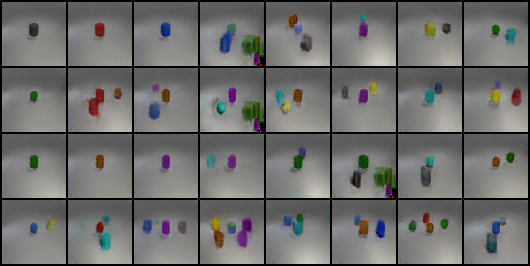
\includegraphics[width=\textwidth]{img/test_w0.5.png}
		\caption{Results of test.json with guidance $w$ 0.5.}
		\label{img-test-0.5}
	\end{figure}
	\begin{figure}[H]
		\centering
		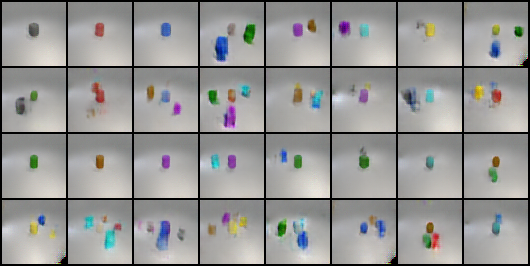
\includegraphics[width=\textwidth]{img/test_w2.0.png}
		\caption{Results of test.json with guidance $w$ 2.0.}
		\label{img-test-2.0}
	\end{figure}
	\begin{figure}[H]
		\centering
		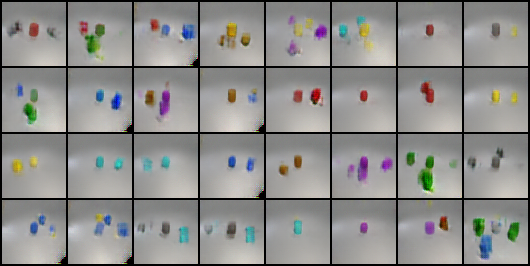
\includegraphics[width=\textwidth]{img/new_test_w0.5.png}
		\caption{Results of new\_test.json with guidance $w$ 0.5.}
		\label{img-new-test-0.5}
	\end{figure}
	\begin{figure}[H]
		\centering
		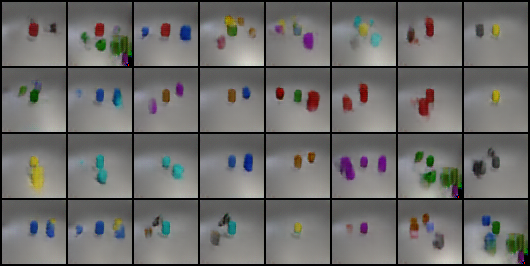
\includegraphics[width=\textwidth]{img/new_test_w2.0.png}
		\caption{Results of new\_test.json with guidance $w$ 2.0.}
		\label{img-new-test-2.0}
	\end{figure}
